\clearpage
\section{CDCE reference isolation: 15 November 2026}
The installed MCU reported PRIMARY/PLL LOCKED. Its normal diagnostic exposes
CDCE register8 only; the attempted read-only ALL argument was rejected.
The reference selector could not be changed through that console interface.
A minimal overlay changed one instruction byte at0xAF9 from EF to E3
(LDI R16,F5 to35), changing the native IRQ's R5 word from40040FF5 automatic
PRI/SEC/AUX to existing40040F35 forced AUX. The instruction encoding was
verified with shared AVR GCC. Native IRQ/power logic and all output dividers
were otherwise unchanged. UART independently confirmed INTERNAL/PLL LOCKED.
R5 words are firmware-derived, not freshly read register5 RAM values.
Reference: \href{https://www.ti.com/lit/ds/symlink/cdce62005.pdf}{TI SCAS862G,
register5 Smart MUX}.

Only bounded application-memory programming was used, with fresh full backup
and exact readback. Bootloader, MCU EEPROM, fuse/lock and signature memories
were compared unchanged. No CDCE EEPROM-copy command was sent. The legacy PC
command was excluded because its original profile includes EEPROM copy.

\subsection{Clock comparison through read-only JTAG}
PM Ethernet stopped responding under AUX, so buffer acquisition through IPbus
could not serve as the independent comparison. Kasli remained at its original
clock and continued to send SPI/read MISO. A read-only USER1 service sampled
the existing SYS counter before and about60ms after each frame, with idle gaps.
RTL increments this counter on SYS and clears it on SYS reset. Modulo32-bit
subtraction handles ordinary wrap; host/JTAG timestamps distinguish normal
20--60MHz advance from a restart. Raw512-bit reports and signatures are retained.
This does not measure analog clock quality or capture every short LOCK pulse.

\begin{center}\begin{tabular}{lrrr}\toprule
Reference & Reads & SYS counter restarts & Correct replies\\\midrule
PRIMARY / HDMI &6&4/6&6/6\\
AUX / local crystal &12&0/12&12/12\\\bottomrule
\end{tabular}\end{center}
Approximate SYS rates were40.079211MHz and39.999998MHz, respectively;
these are uncalibrated counter/time estimates. PRIMARY failures occurred on
reads0/1, while read2 was quiet. All addresses were quiet in the AUX series.
The result supports a relationship with external-reference operation, but does
not isolate cable crosstalk, termination, phase or clock electrical quality.
\begin{center}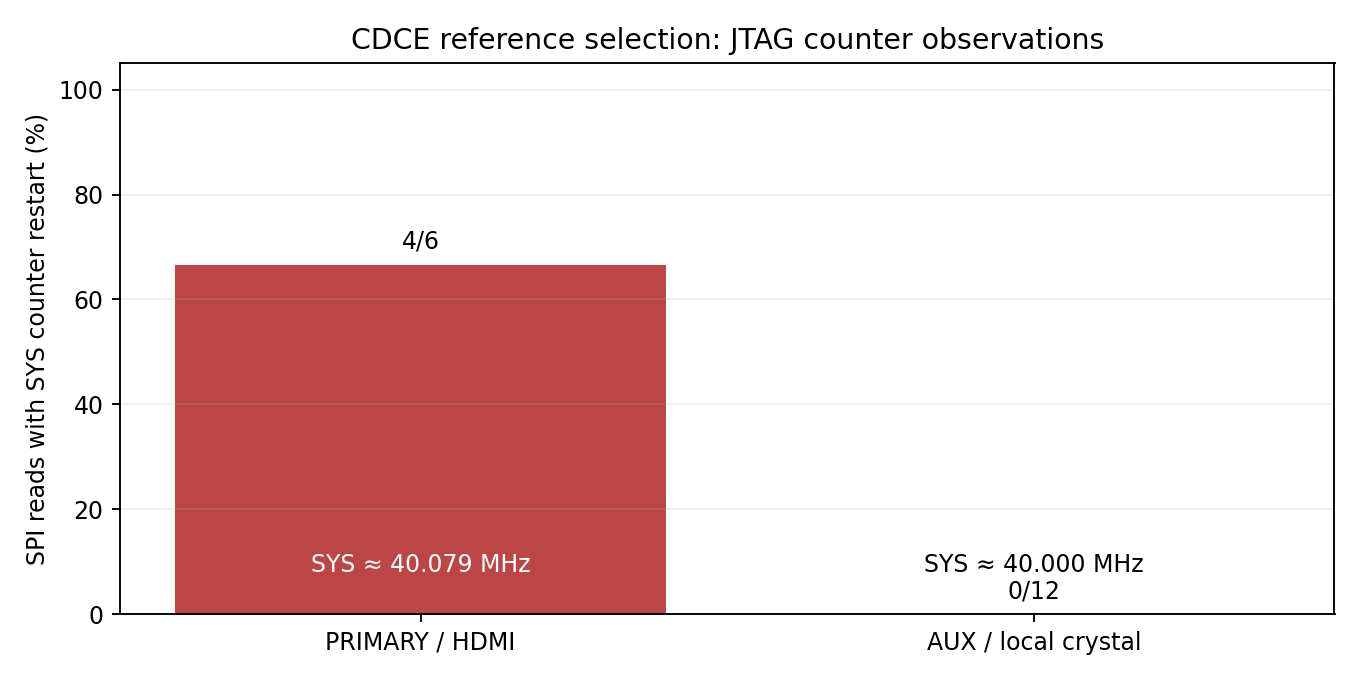
\includegraphics[width=\linewidth]{cdce-aux.png}\end{center}

\subsection{Rejected candidates and final restoration}
AUX could not be accepted as the final operating profile. ADT7311 readback was
all zero after startup in that trial. A separate candidate preserved original
AUTO startup and changed two unused PC operands to select just the existing
R5 AUX word (address0x292E, count1), excluding EEPROM copy. It also returned
zero ADT data on PRIMARY before any PC invocation. The runtime switch was
therefore not executed. This does not establish AUX as the cause of the sensor
initialization failure. The profiles were not fully matched in peripheral state,
so the clock result is diagnostic evidence rather than unconditional acceptance.

The Kasli side remained nominal1.202361Gb/s; PM becomes nominal1.2Gb/s on AUX.
This mismatch is a plausible explanation for loss of PM Ethernet, not separately
proved. PM/Kasli also cease sharing a phase reference. No ADC acquisition or
common-clock phase validation is claimed on AUX.

All overlays were rejected/restored. Final full MCU hash matches the original
\begin{center}\path{f49643c80c6189afebdaa3f7301f4ecebacb55645e60456f66831106d38b9464}\end{center}
Current source is AUTO selecting PRIMARY, PLL LOCKED. FPGA71ac56fb quiet-write
mode4 is restored, PM Ethernet works, frontend readiness0xfff and PGOOD pass,
ADT ID is C3, and all12 physical ADC bank-A captures pass. Kasli outputs stayed
driven and divider600 was restored. The separate read-induced clock fault
remains OPEN. Raw/error cohorts and final restoration receipts:
\begin{center}\path{system/evidence-cdce-aux-20261115}\end{center}
Full MCU/protected-memory backups remain private outside Git; public evidence
contains textual logs/results, raw JTAG words and final restored ADC data.
